%scritto da Federico Perin
\subsubsection{UCA 3 - Gestione lista delle organizzazioni}%kite level
\begin{figure}[h]
	\centering
	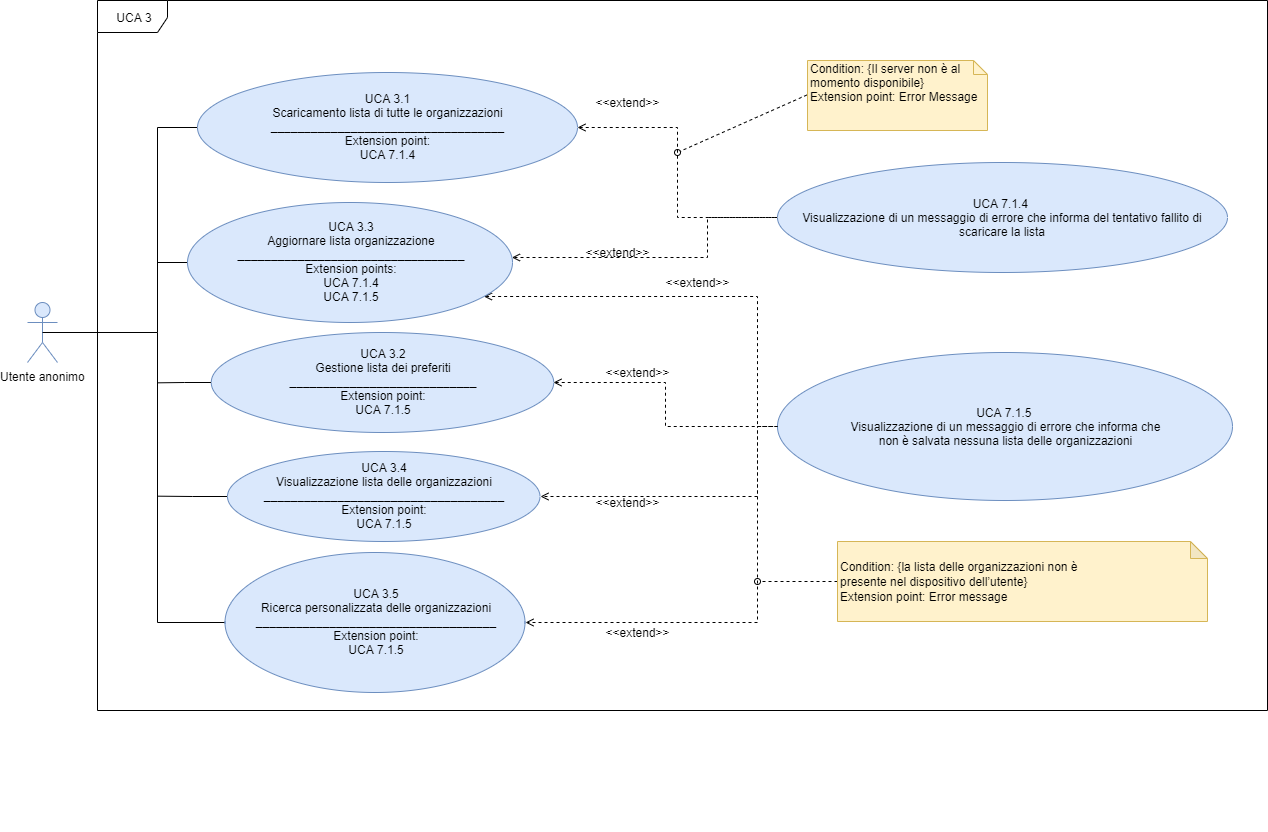
\includegraphics[scale=0.4, left]{sezioni/UseCase/Immagini/UCA3.png}
	\caption{UCA 3 - Gestione lista delle organizzazioni}
\end{figure} 

\begin{itemize}
\item \textbf{Attori primari:} Utente anonimo
\item \textbf{Precondizione:} L'utente è autenticato e può accedere alle funzionalità della lista delle organizzazioni\ap{G}.
\item \textbf{Postcondizione:} Vengono forniti all'utente i risultati delle funzionalità disponibili.
\item \textbf{Scenario principale:} L'utente autenticato utilizza le funzioni di gestione delle liste di organizzazioni\ap{G} per svolgere una o più delle seguenti azioni:
	\begin{itemize}
		\item Scaricamento lista di tutte le organizzazioni\ap{G} [UCA 3.1];
		\item Gestione lista delle organizzazioni preferite\ap{G} [UCA 3.2];
		\item Aggiornare lista organizzazione\ap{G} [UCA 3.3];
		\item Visualizzazione lista delle organizzazioni [UCA 3.4];
		\item Ricerca personalizzata delle organizzazioni\ap{G} [UCA 3.5].
	\end{itemize}
\end{itemize}

\subsubsection{UCA 3.1 - Scaricamento lista di tutte le organizzazioni}%sea level
\begin{itemize}
\item \textbf{Attori primari:} Utente anonimo
\item \textbf{Precondizione:} L'utente è autenticato e può scaricare la lista di tutte le organizzazioni\ap{G}.
\item \textbf{Postcondizione:} L'utente ha a disposizione la lista di tutte le organizzazioni\ap{G}.
\item \textbf{Scenario principale:} L'utente seleziona l'esecuzione della funzione "Scaricamento della lista".
\item \textbf{Scenario alternativo:} Se il tentativo di scaricare la lista fallisce viene visualizzato all'utente un messaggio di errore che lo informa di tale problema [UCA 7.3.1].
\item \textbf{Estensioni:}
	\begin{itemize}
	\item UCA 7.3.1 - Visualizzazione di un messaggio di errore che informa del tentativo fallito di scaricare la lista.
\end{itemize}
  
\end{itemize}

\subsubsection{UCA 3.2 - Gestione lista delle organizzazioni preferite}%sea level
\begin{figure}[h]
	\centering
	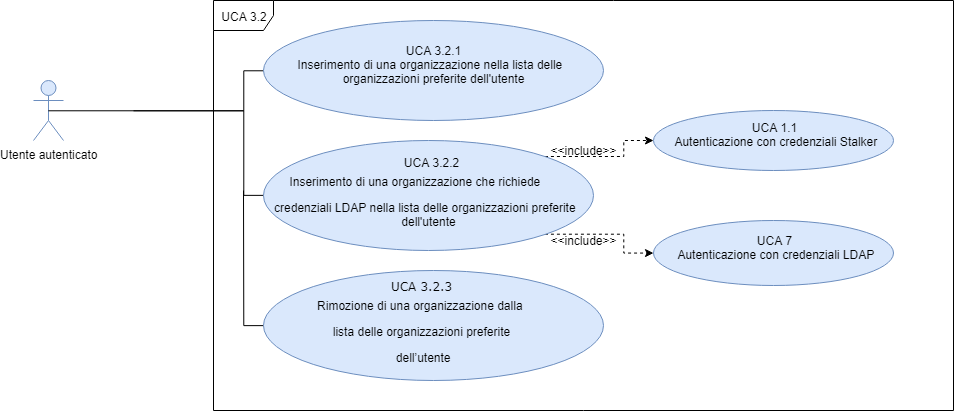
\includegraphics[scale=0.5]{sezioni/UseCase/Immagini/UCA3.2.png}
	\caption{UCA 3.2 - Gestione lista delle organizzazioni preferite}
\end{figure}
\begin{itemize}
	\item \textbf{Attori primari:} Utente anonimo
	\item \textbf{Precondizione:} L'utente è autenticato e può gestire la propria lista delle organizzazioni preferite\ap{G}.
	\item \textbf{Postcondizione:} All'utente vengono forniti i risultati delle funzionalità disponibili.
	\item \textbf{Scenario principale:} L'utente autenticato ha selezionato la funzionalità di gestione della lista delle organizzazioni preferite\ap{G}.
	\item \textbf{Flusso di eventi:}
			\begin{enumerate}
			\item L'utente accede alla funzionalità di "Gestioni della lista delle organizzazioni preferite\ap{G}";
			\item Vi è la possibilità di inserire un'organizzazione\ap{G} nella lista delle organizzazioni preferite\ap{G} dell'utente dell'applicazione [UCA 3.2.1], se però viene richiesto di inserire una organizzazione\ap{G} che richiede di autenticarsi con credenziali LDAP\ap{G} [UCA 3.2.2] allora l'utente dovrà inserire tali credenziali [UCA 1.1];
			\item Vi è la possibilità di rimuovere un'organizzazione\ap{G} dalla lista delle organizzazioni preferite\ap{G} dell'utente dell'applicazione [UCA 3.2.3].
			\end{enumerate}
	\item \textbf{Scenario alternativo:} Se non è presente nessuna lista delle organizzazioni\ap{G} viene visualizzato all'utente un messaggio di errore che lo informa di tale problema [UCA 7.3.2];
	\item \textbf{Estensioni:}
	\begin{itemize}
		\item UCA 7.3.2 - Visualizzazione di un messaggio di errore che informa che non è salvata nessuna lista delle organizzazioni\ap{G}.
	\end{itemize}
\end{itemize}

\subsubsection{UCA 3.2.1 - Inserimento di una organizzazione nella lista delle organizzazioni preferite dell'utente dell'applicazione}%fish level
\begin{itemize}
	\item \textbf{Attori primari:} Utente anonimo
	\item \textbf{Precondizione:} L'utente è autenticato sceglie di eseguire la funzionalità di inserimento di un'organizzazione nella lista delle organizzazioni preferite\ap{G} (solo se ha scaricato precedentemente la lista delle organizzazioni\ap{G}).
	\item \textbf{Postcondizione:} È stata inserita un'organizzazione\ap{G}, scelta dall'utente, nella lista delle organizzazioni preferite\ap{G}.
	\item \textbf{Flusso di eventi:}
	\begin{enumerate}
		\item L'utente seleziona dalla lista delle organizzazioni\ap{G} l'organizzazione\ap{G} da inserire nella lista delle organizzazioni preferite\ap{G};
		\item L'utente conferma l'inserimento nella lista delle organizzazioni preferite\ap{G} per l'organizzazione\ap{G} scelta.
	\end{enumerate}
\end{itemize}

\subsubsection{UCA 3.2.2 - Inserimento di una organizzazione che richiede credenziali LDAP nella lista delle organizzazioni preferite dell'utente dell'applicazione}%fish level
\begin{itemize}
	\item \textbf{Attori primari:} Utente anonimo
	\item \textbf{Precondizione:} L'utente è autenticato e sceglie di eseguire la funzionalità di inserimento nella lista delle organizzazioni preferite\ap{G} solo se ha scaricato precedentemente la lista delle organizzazioni\ap{G}.
	\item \textbf{Postcondizione:} È stata inserita un'organizzazione\ap{G}, scelta dall'utente, nella lista delle organizzazioni preferite\ap{G}.
	\item \textbf{Flusso di eventi:}
	\begin{enumerate}
		\item L'utente seleziona dalla lista delle organizzazioni\ap{G} l'organizzazione\ap{G} da inserire nella lista delle organizzazioni preferite\ap{G};
		\item L'utente conferma l'inserimento nella lista delle organizzazioni preferite\ap{G} per l'organizzazione\ap{G} scelta;
		\item L'utente si autentica con credenziali LDAP\ap{G}.
	\end{enumerate}
	\item \textbf{Inclusioni:}
	\begin{itemize}
			\item UCA - 7 Autenticazione con credenziali LDAP.
	\end{itemize}
\end{itemize}

\subsubsection{UCA 3.2.3 - Rimozione di una organizzazione dalla lista delle organizzazioni preferite dell'utente dell'applicazione}%fish level
\begin{itemize}
	\item \textbf{Attori primari:} Utente anonimo
	\item \textbf{Precondizione:}  L'utente è autenticato sceglie di eseguire la funzionalità di rimozione nella lista delle organizzazioni preferite\ap{G} solo se c'è almeno una organizzazione\ap{G} inserita nella lista delle organizzazioni preferite\ap{G}.
	\item \textbf{Postcondizione:} È stata rimossa l'organizzazione\ap{G}, scelta dall'utente, dalla lista delle organizzazioni preferite\ap{G}.
	\item \textbf{Flusso di eventi:}
	\begin{enumerate}
		\item L'utente seleziona nella lista delle organizzazioni preferite\ap{G} l'organizzazione\ap{G} da rimuovere dalla lista delle organizzazioni preferite\ap{G};
		\item L'utente conferma la rimozione dalla lista delle organizzazioni preferite\ap{G} per l'organizzazione\ap{G} scelta.
	\end{enumerate}
\end{itemize}

\subsubsection{UCA 3.3 - Aggiornare lista organizzazione}%sea level

\begin{figure}[h]
	\centering
	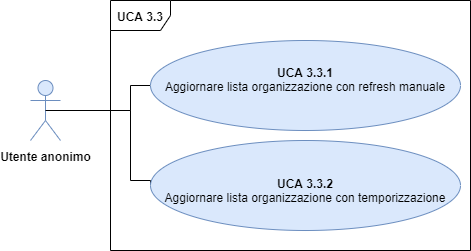
\includegraphics[scale=0.5]{sezioni/UseCase/Immagini/UCA3.3.png}
	\caption{UCA 3.3 - Aggiornare lista organizzazione}
\end{figure}

\begin{itemize} 
	\item \textbf{Attori primari:} Utente anonimo
	\item \textbf{Precondizione:} L'utente è autenticato e può aggiornare la lista delle organizzazioni\ap{G}.
	\item \textbf{Postcondizione:} L'utente ha aggiornato la lista di tutte le organizzazioni\ap{G}.
	\item \textbf{Scenario principale:} L'utente ha la necessità di aggiornare la lista e può farlo in diversi modi.
	\item \textbf{Flusso di eventi:}
	\begin{enumerate}
		\item L'utente accede alla funzionalità di aggiornamento della lista delle organizzazioni \ap{G};
		\item L'utente ha la possibilità di effettuare l'aggiornamento lista organizzazione\ap{G} con refresh manuale\ap{G} [UCA 3.3.1];
		\item L'utente ha la possibilità di effettuare l'aggiornamento lista organizzazione\ap{G} con temporizzazione\ap{G} [UCA 3.3.2].
	\end{enumerate}
	\item \textbf{Scenario alternativo 1:} Se il tentativo di scaricare la lista fallisce viene visualizzato all'utente un messaggio di errore che lo informa di tale problema [UCA 7.3.1].
	\item \textbf{Scenario alternativo 2:} Se non è presente nessuna lista delle organizzazioni\ap{G} viene visualizzato all'utente un messaggio di errore che lo informa di tale problema [UCA 7.3.2];
	\item \textbf{Estensioni:}
	\begin{itemize}
		\item UCA 7.3.1 - Visualizzazione di un messaggio di errore che informa del tentativo fallito di scaricare la lista;
		\item UCA 7.3.2 - Visualizzazione di un messaggio di errore che informa che non è salvata nessuna lista delle organizzazioni\ap{G}.
	\end{itemize}
\end{itemize}

\subsubsection{UCA 3.3.1 - Aggiornare lista organizzazione con refresh manuale}%fish level
\begin{itemize}
	\item \textbf{Attori primari:} Utente anonimo
	\item \textbf{Precondizione:} L'utente anonimo sceglie di eseguire la funzionalità aggiornamento della lista dell'organizzazione\ap{G} attraverso la modalità di refresh manuale\ap{G}.
	\item \textbf{Postcondizione:} La lista delle organizzazioni\ap{G} è aggiornata.	
	\item \textbf{Flusso di eventi:}
	\begin{enumerate}
		\item L'utente esegue l'aggiornamento della lista delle organizzazioni\ap{G} attraverso un refresh manuale\ap{G}.
	\end{enumerate}
	
\end{itemize}

\subsubsection{UCA 3.3.2 - Aggiornare lista organizzazione con temporizzazione}%fish level
\begin{itemize} 
	\item \textbf{Attori primari:} Utente anonimo
	\item \textbf{Precondizione:} L'utente anonimo sceglie di eseguire la funzionalità aggiornamento della lista dell'organizzazione\ap{G} attraverso la modalità temporizzazione\ap{G}.
	\item \textbf{Postcondizione:} La lista delle organizzazioni è aggiornata.
	\item \textbf{Flusso di eventi:}
	\begin{enumerate}
		\item L'utente esegue l'aggiornamento della lista dell'organizzazione\ap{G} attraverso la modalità temporizzazione\ap{G}.
	\end{enumerate}
\end{itemize}

\subsubsection{UCA 3.4 - Visualizzazione lista delle organizzazioni}%sea level

\begin{figure}[h]
	\centering	
	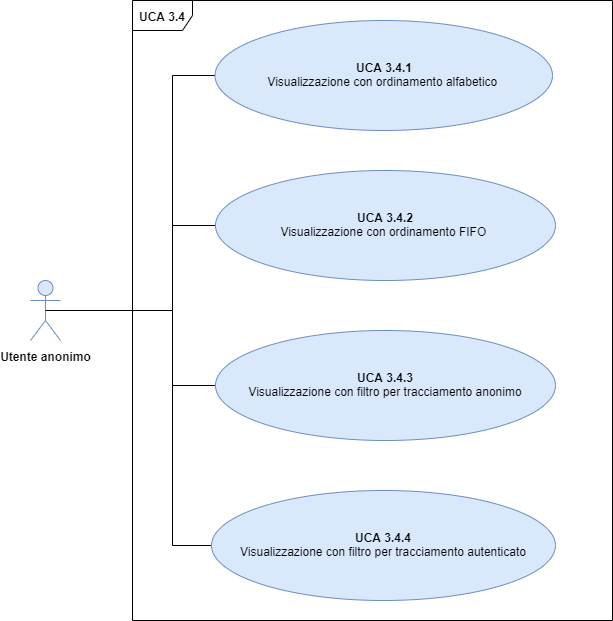
\includegraphics[scale=0.5]{sezioni/UseCase/Immagini/UCA3.4.png}
	\caption{UCA 3.4 - Visualizzazione lista delle organizzazioni}
\end{figure}

\begin{itemize} 
	\item \textbf{Attori primari:} Utente anonimo
	\item \textbf{Precondizione:}  L'utente è autenticato e può visualizzare la lista delle organizzazioni\ap{G}.
	\item \textbf{Postcondizione:} L'utente visualizza la lista delle organizzazioni\ap{G} nel modo che ritiene più opportuno.
	\item \textbf{Scenario principale:}	L'utente può scegliere come visualizzare la lista tra diversi tipi di ordinamento.
	\item \textbf{Flusso di eventi:}
	\begin{enumerate}
		\item L'utente esegue la funzione per la visualizzazione della lista, visualizzando i nomi delle organizzazioni\ap{G} presenti;
		\item L'utente ha la possibilità di ordinare le organizzazioni\ap{G} alfabeticamente [UCA 3.4.1];
		\item L'utente ha la possibilità di ordinare le organizzazioni\ap{G} secondo la politica FIFO\ap{G} [UCA 3.4.2];
		\item L'utente ha la possibilità di applicare un filtro per modalità di tracciamento anonima\ap{G} [UCA 3.4.3];
		\item L'utente ha la possibilità di applicare un filtro per modalità di tracciamento autenticato\ap{G} [UCA 3.4.4].
	\end{enumerate}
	\item \textbf{Scenario alternativo:} Se non è presente nessuna lista delle organizzazioni\ap{G} viene visualizzato all'utente un messaggio di errore che lo informa di tale problema.
	\item \textbf{Estensioni:}
	\begin{itemize}
		\item UCA 7.3.2 - Visualizzazione di un messaggio di errore che informa che non è salvata nessuna lista delle organizzazioni\ap{G}.
	\end{itemize}
\end{itemize}

\subsubsection{UCA 3.4.1 - Visualizzazione con ordinamento alfabetico}%fish level
\begin{itemize}
	\item \textbf{Attori primari:} Utente anonimo
	\item \textbf{Precondizione:} L'utente autenticato può utilizzare la funzionalità di visualizzazione della lista secondo un ordinamento alfabetico (dalla a alla z) per il nome dell'organizzazione\ap{G}.
	\item \textbf{Postcondizione:} Viene visualizzata la lista delle organizzazioni\ap{G} in ordine alfabetico per il nome dell'organizzazione\ap{G}.
	\item \textbf{Flusso di eventi:}
	\begin{enumerate}
		\item L'utente esegue la funzione per la visualizzazione della lista, visualizzando i nomi delle organizzazioni\ap{G} presenti in ordine alfabetico.
	\end{enumerate}
\end{itemize}

\subsubsection{UCA 3.4.2 - Visualizzazione con ordinamento FIFO}%fish level
\begin{itemize}	
	\item \textbf{Attori primari:} Utente anonimo
	\item \textbf{Precondizione:} L'utente autenticato può utilizzare la funzionalità di visualizzazione della lista secondo un ordinamento FIFO\ap{G}.
	\item \textbf{Postcondizione:} Viene visualizzato la lista delle organizzazioni\ap{G} secondo un ordinamento FIFO\ap{G}.
	\item \textbf{Flusso di eventi:}
		\begin{enumerate}
		\item L'utente esegue la funzione per la visualizzazione della lista, visualizzando i nomi delle organizzazioni\ap{G} presenti secondo un ordinamento FIFO\ap{G}.
	\end{enumerate}
\end{itemize}

\subsubsection{UCA 3.4.3 - Visualizzazione con filtro per tracciamento anonimo}%fish level
\begin{itemize}
	\item \textbf{Attori primari:} Utente anonimo
	\item \textbf{Precondizione:} L'utente autenticato può utilizzare la funzionalità di visualizzazione della lista che permettono un tracciamento anonimo\ap{G}.
	\item \textbf{Postcondizione:} Viene visualizzato la lista delle organizzazioni\ap{G} che richiedono il tracciamento anonimo\ap{G}.
	\item \textbf{Flusso di eventi:}
		\begin{enumerate}
		\item L'utente esegue la funzione per la visualizzazione della lista, visualizzando i nomi delle organizzazioni\ap{G} che permettono il tracciamento anonimo\ap{G}.
	\end{enumerate}
\end{itemize}

\subsubsection{UCA 3.4.4 - Visualizzazione con filtro per tracciamento autenticato}%fish level
\begin{itemize}
	\item \textbf{Attori primari:} Utente anonimo
	\item \textbf{Precondizione:} L'utente autenticato può utilizzare la funzionalità di visualizzazione della lista che permette un tracciamento autenticato\ap{G}.
	\item \textbf{Postcondizione:} Viene visualizzato la lista delle organizzazioni\ap{G} che permettono il tracciamento autenticato\ap{G}.
	\item \textbf{Flusso di eventi:}
	\begin{enumerate}
		\item L'utente esegue la funzione per la visualizzazione della lista, visualizzando i nomi delle organizzazioni\ap{G} che permettono il tracciamento autenticato\ap{G}.
	\end{enumerate}
\end{itemize}

\subsubsection{UCA 3.5 - Ricerca personalizzata delle organizzazioni}%sea level
\begin{figure}[h]
	\centering
	
	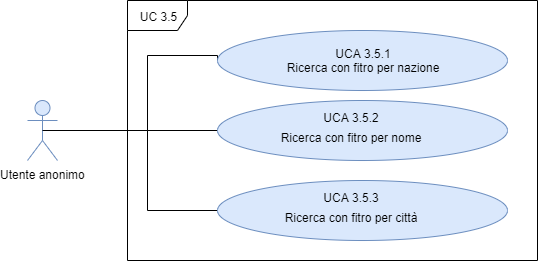
\includegraphics[scale=0.5]{sezioni/UseCase/Immagini/UCA3.5.png}
	\caption{UCA 3.5 - Ricerca personalizzata delle organizzazioni}
\end{figure}
\begin{itemize}
	\item \textbf{Attori primari:} Utente anonimo
	\item \textbf{Precondizione:} L'utente è autenticato e può svolgere ricerche riguardo le organizzazioni\ap{G}.
	\item \textbf{Postcondizione:} Vengono forniti all'utente i risultati delle ricerche.
	\item \textbf{Scenario principale:} L'utente deve svolgere alcune ricerche e sceglie il metodo che più lo aggrada.
	\item \textbf{Flusso di eventi:} 
	\begin{enumerate}
		\item L'utente anonimo accede alla funzionalità di ricerca personalizzata della lista delle organizzazioni\ap{G} per ricercare le organizzazioni\ap{G} desiderate;
		\item L'utente ha la possibilità di effettuare la ricerca per nazione [UCA 3.5.1];
		\item L'utente ha la possibilità di effettuare la ricerca per nome [UCA 3.5.2];
		\item L'utente ha la possibilità di effettuare la ricerca per città [UCA 3.5.3].
	\end{enumerate}
	\item \textbf{Scenario alternativo:} Se non è presente nessuna lista delle organizzazioni viene visualizzato all'utente un messaggio di errore che lo informa di tale problema [UCA 7.3.2].
	\item \textbf{Estensioni:}
	\begin{itemize}
		\item UCA 7.3.2 - Visualizzazione di un messaggio di errore che informa che non è salvata nessuna lista delle organizzazioni\ap{G}.
	\end{itemize}
\end{itemize}

\subsubsection{UCA 3.5.1 - Ricerca con filtro per nazione}%fish level
\begin{itemize}
	\item \textbf{Attori primari:} Utente anonimo
	\item \textbf{Precondizione:} L'utente autenticato può utilizzare la funzionalità di ricerca della lista per cercare le organizzazioni\ap{G} di una certa nazione d'interesse.
	\item \textbf{Postcondizione:} Viene visualizzato la lista delle organizzazioni\ap{G} che sono nella nazione scelta dall'utente.
	\item \textbf{Flusso di eventi:}
	\begin{enumerate}
		\item L'utente esegue la funzione di ricerca personalizzata della lista delle organizzazioni\ap{G} per ricercare le organizzazioni\ap{G} desiderate, filtrando per la nazione scelta.
	\end{enumerate}
\end{itemize}

\subsubsection{UCA 3.5.2 - Ricerca con filtro per nome}%fish level
\begin{itemize}
	\item \textbf{Attori primari:} Utente anonimo
	\item \textbf{Precondizione:} L'utente autenticato può utilizzare la funzionalità di ricerca della lista per cercare le organizzazioni\ap{G} che hanno nel nome una sottostringa specificata dall'utente.
	\item \textbf{Postcondizione:} Viene visualizzato la lista delle organizzazioni\ap{G} che hanno nel nome una sottostringa scelta dall'utente.
	\item \textbf{Flusso di eventi:}
	\begin{enumerate}
		\item L'utente esegue la funzione di ricerca personalizzata della lista delle organizzazioni\ap{G} per ricercare le organizzazioni\ap{G} desiderate, filtrando per il nome della organizzazione scelta.
	\end{enumerate}
\end{itemize}

\subsubsection{UCA 3.5.3 - Ricerca con filtro per città}%fish level
\begin{itemize}
	\item \textbf{Attori primari:} Utente anonimo
	\item \textbf{Precondizione:} L'utente autenticato può utilizzare la funzionalità di ricerca della lista per cercare le organizzazioni\ap{G} di una certa città d'interesse.
	\item \textbf{Postcondizione:} Viene visualizzato la lista delle organizzazioni\ap{G} che sono nella città scelta dall'utente.
	\item \textbf{Flusso di eventi:}
	\begin{enumerate}
		\item L'utente esegue la funzione di ricerca personalizzata della lista delle organizzazioni\ap{G} per ricercare le organizzazioni\ap{G} desiderate, filtrando per la città scelta.
	\end{enumerate}
\end{itemize}